%**************** KARATE CLUB DATASET APPLICATION ******************
\section{Application to Zachary's Karate Club Graph}
\label{sec5.3}

Zachary’s Karate Club is a classic social network collected by Wayne Zachary in the 1970s ~\cite{ZacharyKarateClubGraph}. It represents the relationships among 34 members of a university karate club, where each node is a person and an edge indicates some kind of social interaction (e.g., friendship or frequent contact) between two members. During the study, the karate club split into two factions due to an internal dispute, effectively dividing the network into two communities.

Therefore, our goal was to apply the Ricci Flow method to the graph in order to identify these two distinct communities.
Fig.~\ref{fig:Karate_comparison_graphs_a} is a plot of the initial graph as loaded from NetwrokX, with edges' colours based on curvature values. In contrast, fig.~\ref{fig:Karate_comparison_graphs_b} shows the same graph after Ricci Flow process, with updated curvature values. 
\begin{figure}
    \centering
    \begin{subfigure}{0.45\textwidth}
        \centering
        \includegraphics[width=\textwidth]{../KarateClubResults/Before Ricci Flow (graph).png}
        \caption{Initial Karate graph, before Ricci Flow.}
        \label{fig:Karate_comparison_graphs_a}
    \end{subfigure}
    \hfill
    \begin{subfigure}{0.45\textwidth}
        \centering
        \includegraphics[width=\textwidth]{../KarateClubResults/After Ricci Flow (graph).png}
        \caption{Karate graph after Ricci Flow.}
        \label{fig:Karate_comparison_graphs_b}
    \end{subfigure}
    \caption{Comparison of Karate graph before and after having applied Ricci Flow on edges.}
\end{figure}

As anticipated in the previous section, we added a histogram visualization for a better glimpse on curvatures and also on weights values. The original Ricci curvatures and weights can be seen in fig.~\ref{fig:Karate_comparison_histo_a}, while the updated ones are in fig.~\ref{fig:Karate_comparison_histo_b}.
\begin{figure}
    \centering
    \begin{subfigure}{0.45\textwidth}
        \centering
        \includegraphics[width=\textwidth]{../KarateClubResults/Before Ricci Flow.png}
        \caption{Initial Karate graph, before Ricci Flow.}
        \label{fig:Karate_comparison_histo_a}
    \end{subfigure}
    \hfill
    \begin{subfigure}{0.45\textwidth}
        \centering
        \includegraphics[width=\textwidth]{../KarateClubResults/After Ricci Flow.png}
        \caption{Karate graph after Ricci Flow.}
        \label{fig:Karate_comparison_histo_b}
    \end{subfigure}
    \caption{Comparison of curvature values and weights before and after having applied Ricci Flow on edges.}
\end{figure}

In addition to plotting ARI and modularity with various cutoff thresholds, we also wanted to check the result produced by guessing the cut looking at modularity drops. In fig.~\ref{fig:Karate_Accuracy} the “good cut” guessed as the one corresponding to the maximum before a modularity drop is depicted in red. As we hoped for, it also corresponds to the maximum of ARI, confirming that the method can be still useful in cases in which ground truth is not available.
\begin{figure}
    \centering
    \includegraphics[width=0.6\textwidth]{../KarateClubResults/Surgery Accuracy.png}
    \caption{Karate Club graph's ARI and modularity behavior for different surgery cutoffs. In red is plotted the guessed “good cut” based on the maximum (preceding a drop) of modularity.}
    \label{fig:Karate_Accuracy}
\end{figure}

From fig.~\ref{fig:Karate_Communities_a} we can see the graph after having perform surgery with the best cutoff giving an ARI of $\approx$0.772; which is almost the best result one can get for the Karate Club graph for most of the community detection algorithm ~\cite{Ni:communitydetectionnetworksricci}. To understand better the detected community structure we have them depicted in fig.~\ref{fig:Karate_Communities_b}. Here we can see that only two nodes have been placed in the wrong community.
\begin{figure}
    \centering
    \begin{subfigure}{0.45\textwidth}
        \centering
        \includegraphics[width=\textwidth]{../KarateClubResults/After Surgery.png}
        \caption{Final Karate Club graph, after surgery process.}
        \label{fig:Karate_Communities_a}
    \end{subfigure}
    \hfill
    \begin{subfigure}{0.45\textwidth}
        \centering
        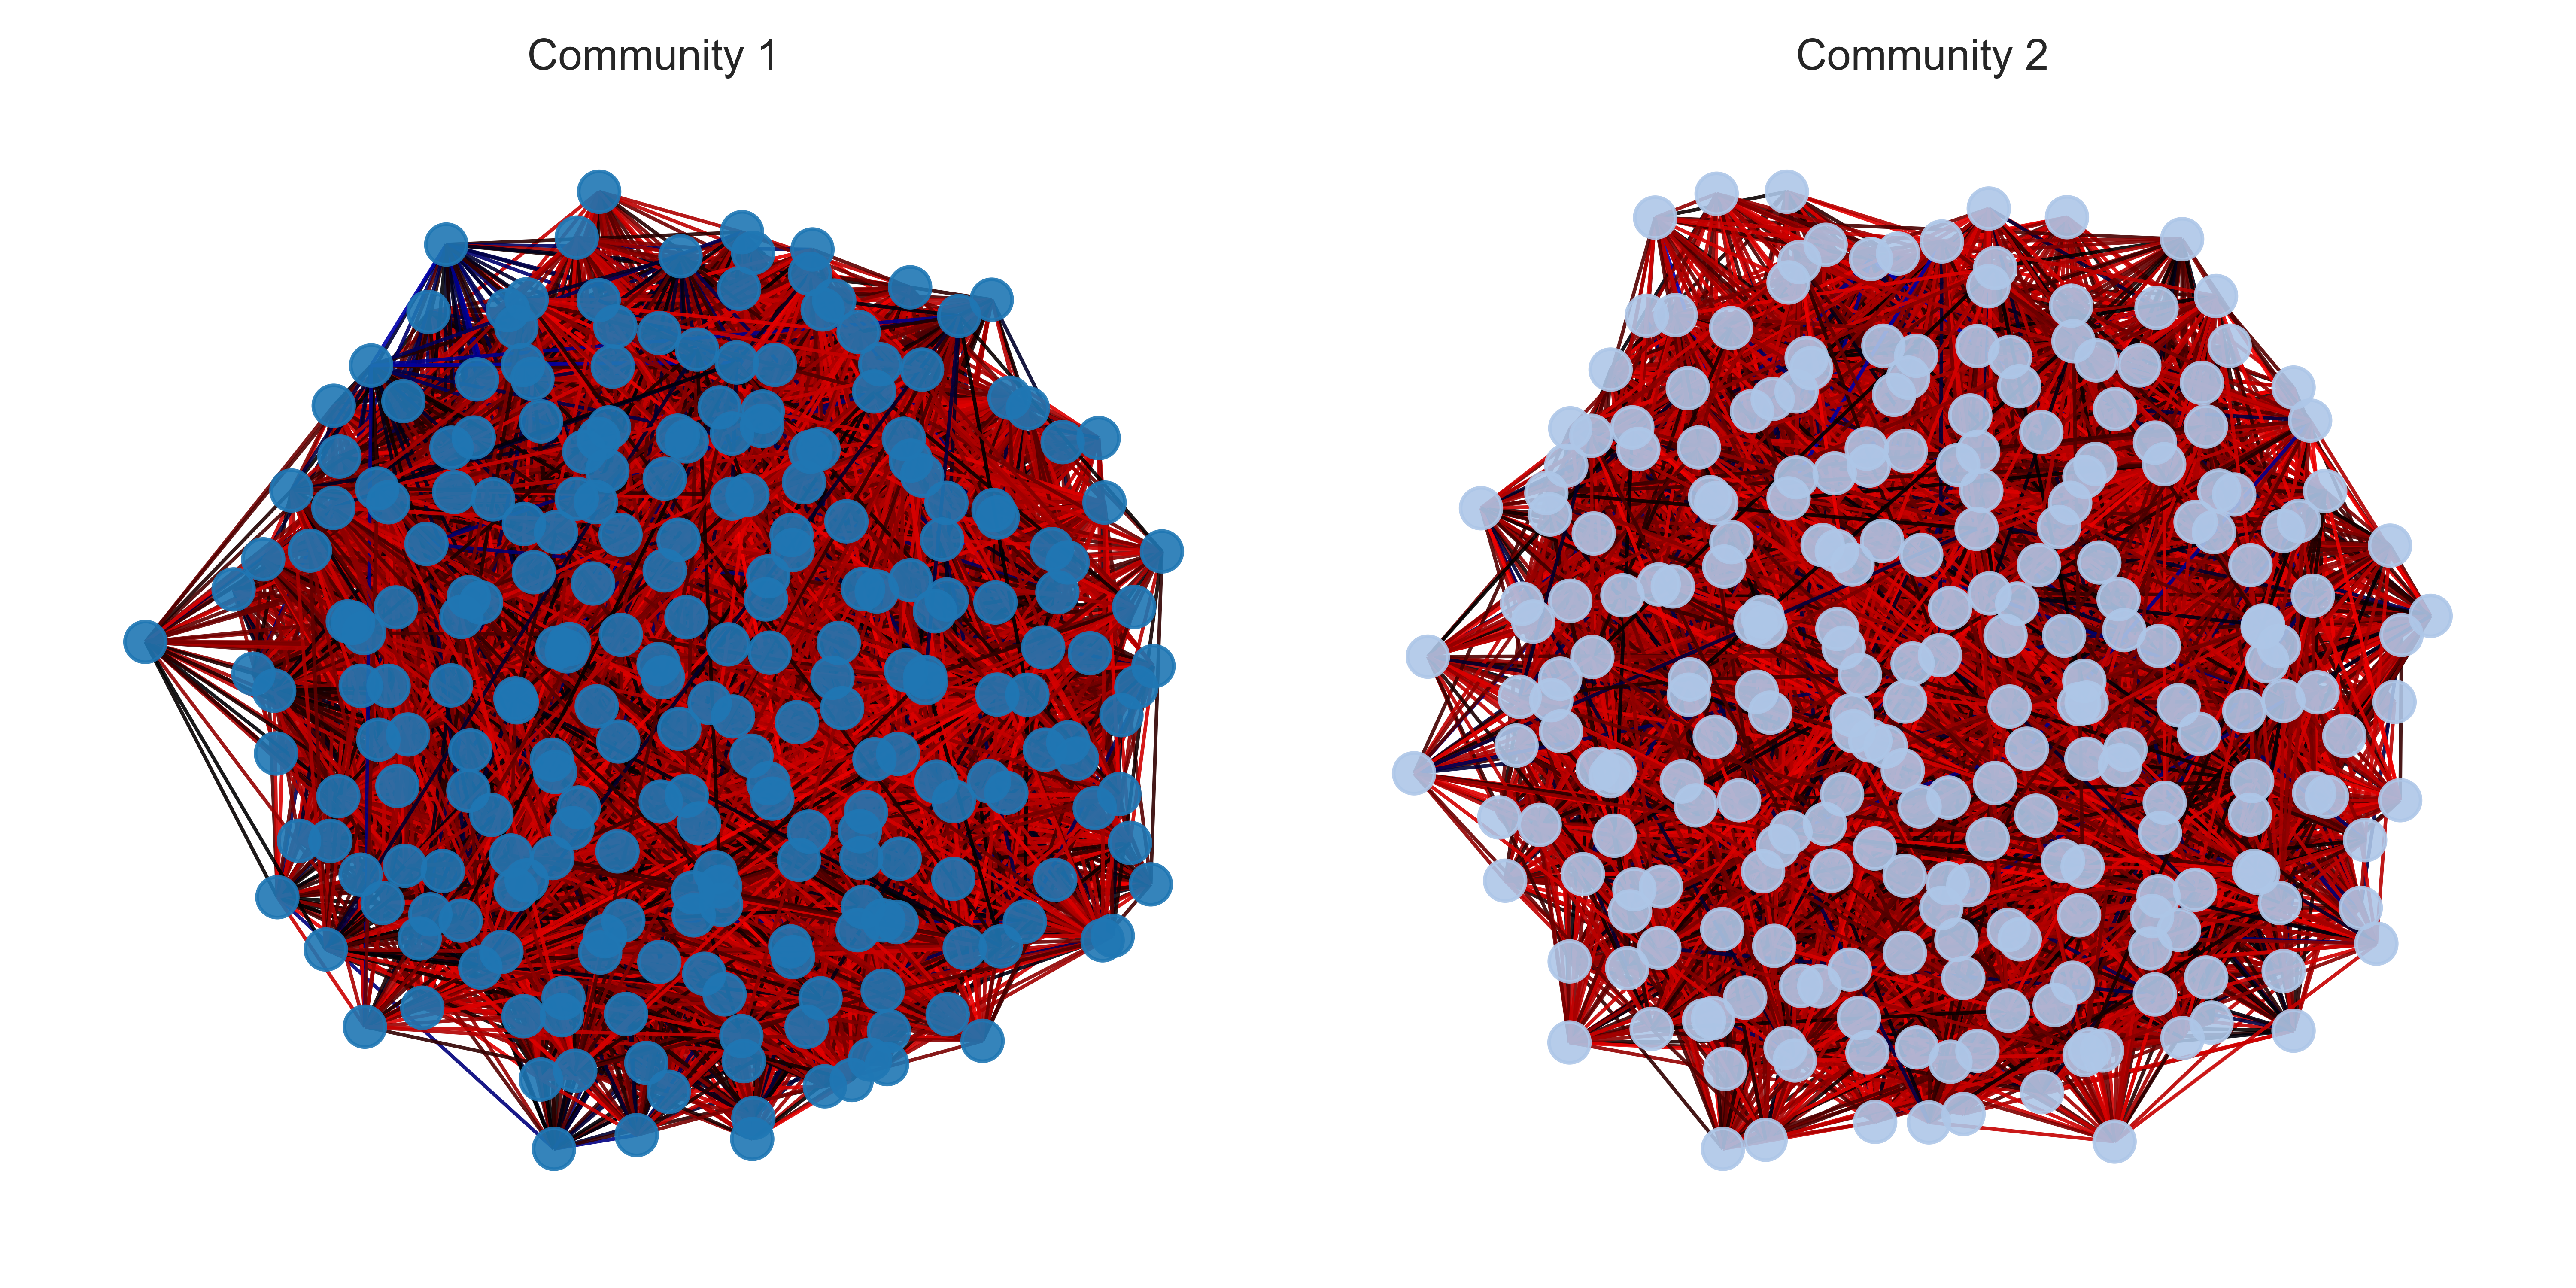
\includegraphics[width=\textwidth]{../KarateClubResults/Detected Communities.png}
        \caption{Detected communities after surgery on Karate Club graph.}
        \label{fig:Karate_Communities_b}
    \end{subfigure}
    \caption{Comparison of Karate graph after surgery and corresponding connected components (i.e., the detected communities).}
\end{figure}

Lastly, we compared the results for ARI and modularity with other two popular community detection algorithms: \textit{Louvian} and \textit{Girvan-Newman}. Results are presented in fig.~\ref{fig:Karate_Comparison}; for modularity obtained from Ricci Flow algorithm we mean the modularity value corresponding to the chosen cutoff for surgery (i.e., modularity at the end of Ricci Flow process, which we recall is evaluated using Louvian method). 

Ricci Flow seems to have transformed the graph in such a way that its modularity has increased, it is higher than the one of the original graph detected by the two other methods. But perhaps the most significant result is that Ricci Flow methods yields a better ARI than Louvian method, which gives only $\approx$0.5, and the same value as Girvan-Newman.
\begin{figure}
    \centering
    \includegraphics[width=\textwidth]{../KarateClubResults/Comparison.png}
    \caption{Karate Club graph comparison in performance between Ricci Flow, Louvian and Girvan-Newman methods.}
    \label{fig:Karate_Comparison}
\end{figure}